\documentclass[12pt,a4paper]{article}
\title{\textbf{Homework2}}
\author{Maedeh Karkhane Yousefi-98100991}
\usepackage{graphicx}
\usepackage{float}
\usepackage{subcaption}
\usepackage{physics}
\begin{document}
\maketitle
\part*{1.Julia Set}

	\paragraph*{}
		For this code I tried creating a 2 dimensional array, filled with zero numbers. In the code I made a loop through an specific range of numbers, representing the real and the imaginary portion of the initial number.  In the innermost loop, the function\textit{$f(z)=z^2+c$} is operated on the point \textit{z}, n times and meanwhile, there is condition checking whether the absolute value of \textit{z} is beyond the boundary (the given formula \textit{$\frac{1+\abs{1+4*\sqrt{\abs{c}}}}{2}$}) or not. There are also two variables representing the x pixel and the y pixel in our resulting image, which are initially set to zero and increase by one after each loop, placing the the absolute value of the final point-if true in the mentioned condition before- in the these specified positions in the array. 
\begin{figure}[H]
	\begin{subfigure}[b]{0.5\textwidth}
		\centering
		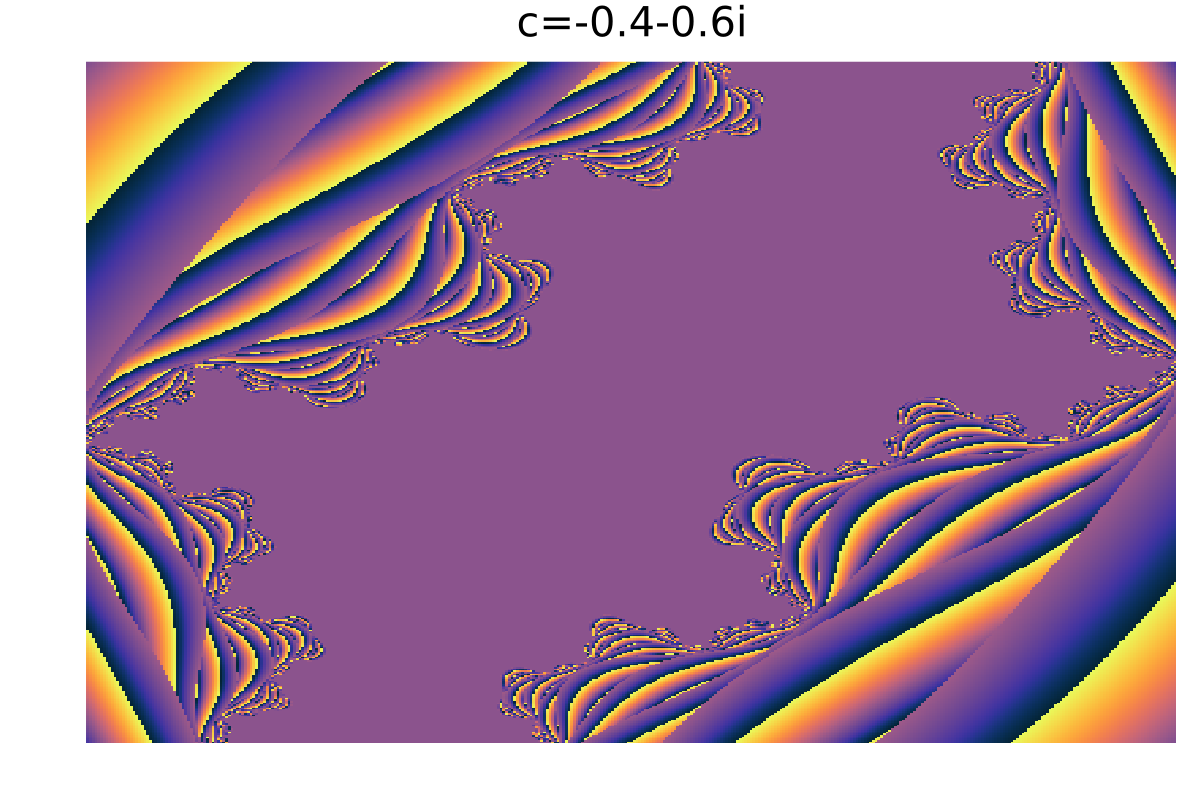
\includegraphics[width=\textwidth]{JuliaSetc1.png}
		\label{fig:1.1}
	\end{subfigure}\hfill
	\begin{subfigure}[b]{0.5\textwidth}
		\centering
		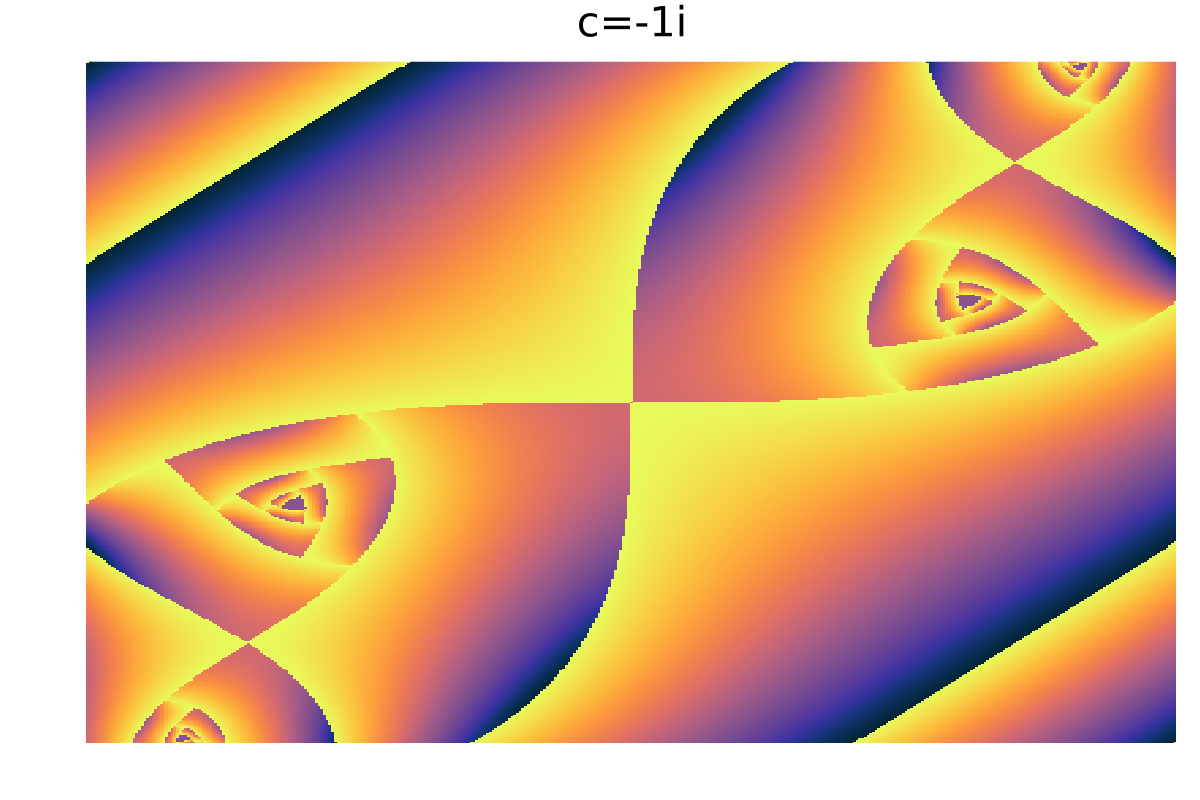
\includegraphics[width=\textwidth]{JuliaSetc2.png}
		\label{fig:1.2}
	\end{subfigure}\hfill
	\begin{subfigure}[b]{0.5\textwidth}
		\centering
		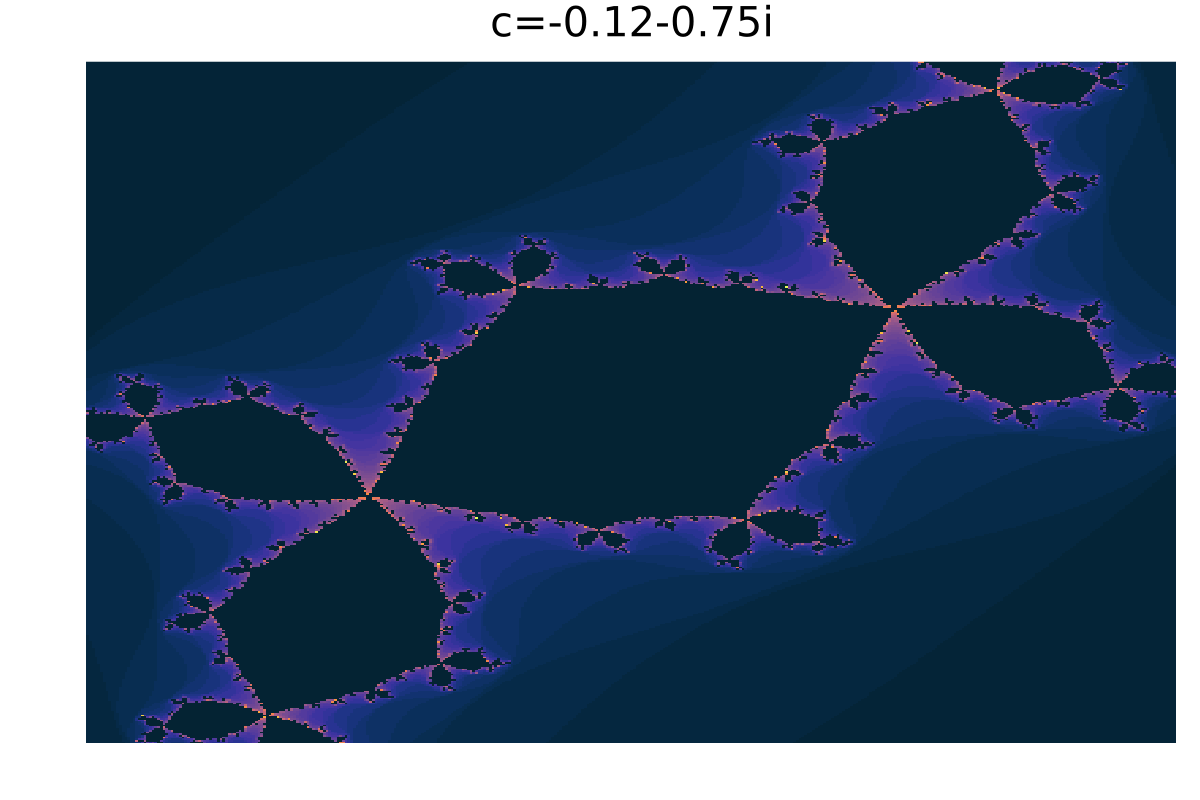
\includegraphics[width=\textwidth]{JuliaSetc3.png}
		\label{fig:1.3}
	\end{subfigure}\hfill
	\begin{subfigure}[b]{0.5\textwidth}
		\centering
		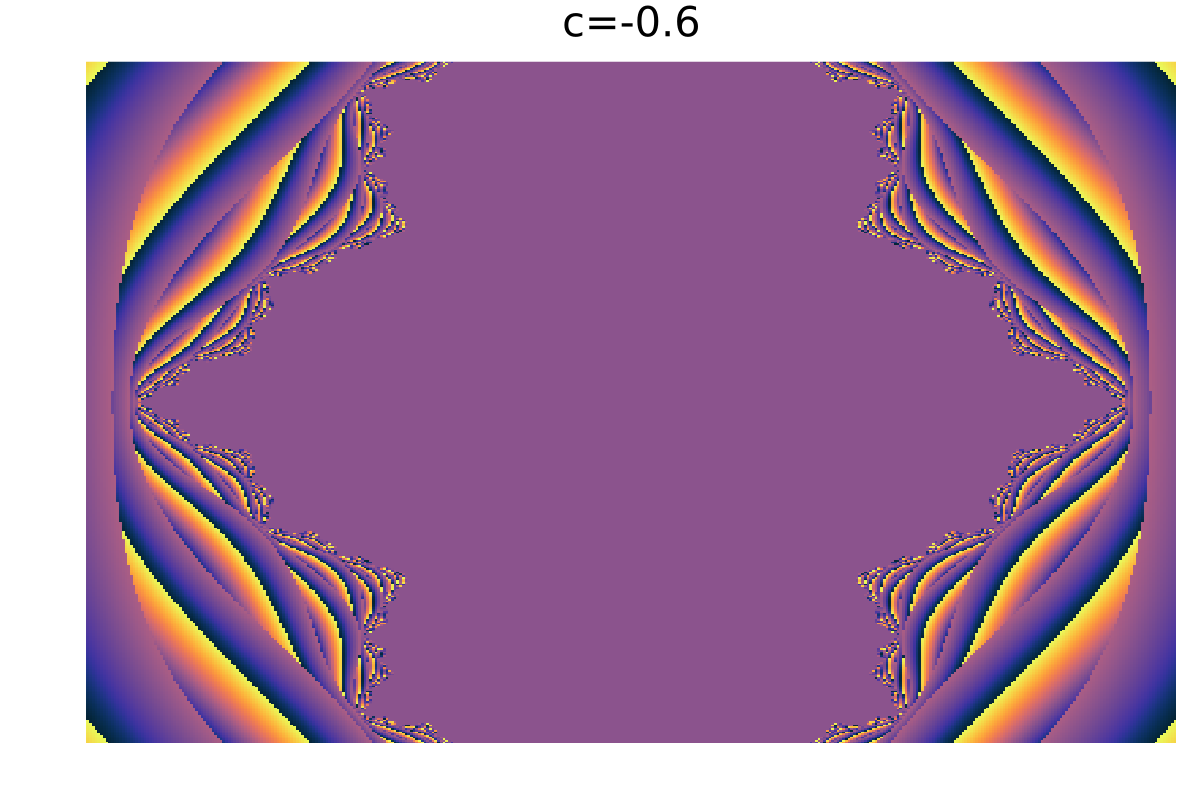
\includegraphics[width=\textwidth]{JuliaSetc4.png}
		\label{fig:1.4}
	\end{subfigure}\hfill
	\begin{subfigure}[b]{0.5\textwidth}
		\centering
		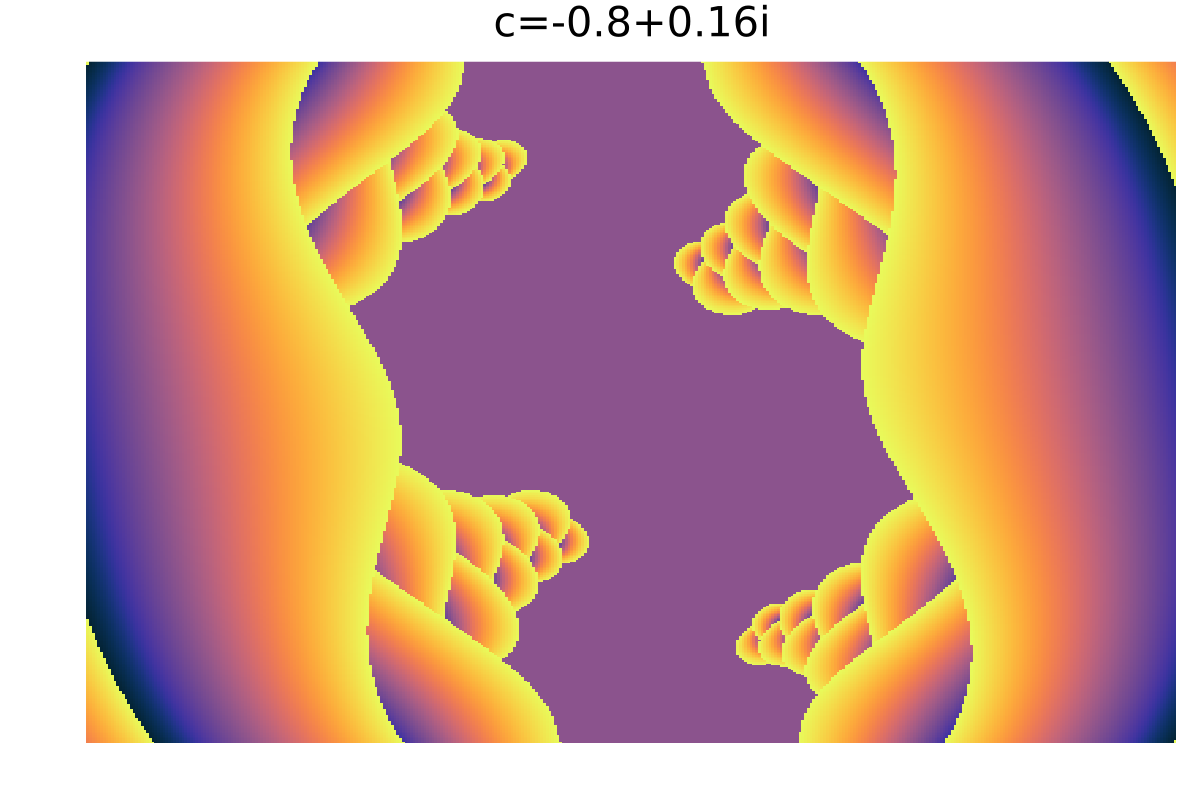
\includegraphics[width=\textwidth]{JuliaSetc5.png}
		\label{fig:1.5}
	\end{subfigure}\hfill
	\begin{subfigure}[b]{0.5\textwidth}
		\centering
		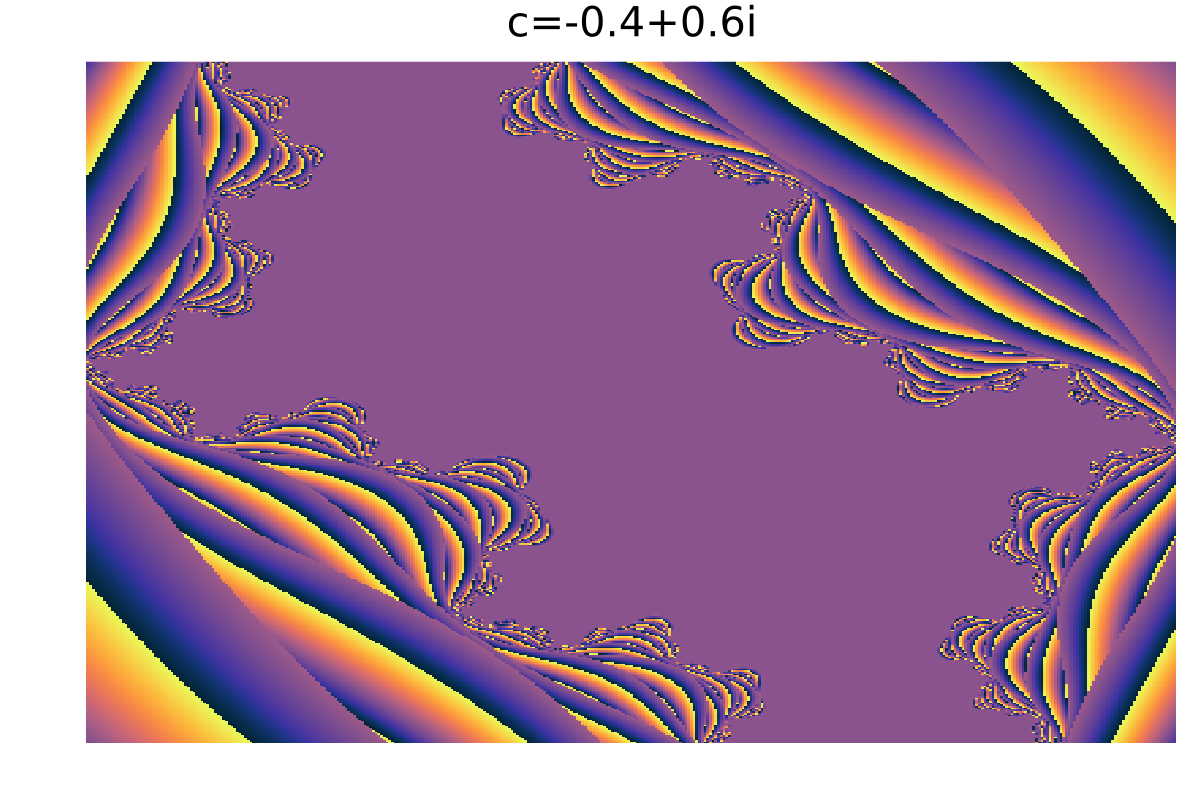
\includegraphics[width=\textwidth]{JuliaSetc6.png}
		\label{fig:1.6}
	\end{subfigure}\hfill
	\label{fig:mesh1}
	\caption{Julia Set is plotted for different values of c. Points are assumed to be between -1-i and 1+i with equal steps of 0.005 between each real and imaginary portion of the point. The function is $f(z)=z^2+c$ and iteration on every point is set to be 10.}
\end{figure}

\part*{2.Random Ballistic Deposition}
\paragraph*{}
	assuming \textit{L} to be the length of the line, I constructed a \textit{L$\times$L array} filled with zero numbers. In a loop through the total number of particles that we aim to sit on the line, in each step we introduce a random number which denotes the column that particle is. In the next loop we check all the rows in that column from bottom to top, for the first entry that is zero, or in the other words, empty. An specific number will be associated to that entry -other than zero-, confirming that pixel's color in our heatmap plot. The color is going to change after every \textit{L$\times$10} step. 
	\\ for plotting the mean hight of the layer in every time step I wrote a function, which counts all the entries in every column that are not empty, namely "are filled with particles ". Hence, the mean hight value can be calculated using the \textit{mean() function} available in the \textit{statistics package} in Julia. 
\begin{figure}[H]
	\centering
	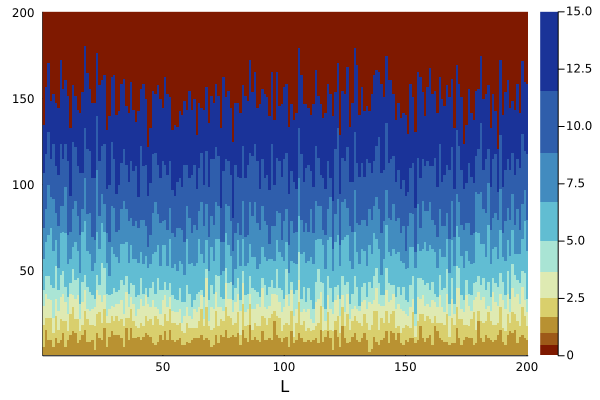
\includegraphics[width=\textwidth]{RandomBallisticDeposition1.png}
	\label{fig:mesh2}
	\caption{The model's dynamic for 30000 particles and a line of L=200 is shown in this plot.}
\end{figure}
\begin{figure}[H]
	\centering
	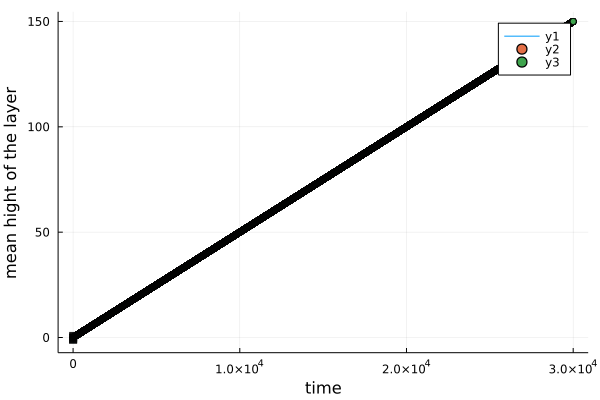
\includegraphics[width=\textwidth]{RandomBallisticDeposition2.png}
	\label{fig:mesh3}
	\caption{Mean Hight of layer over time for 30000 particles and a line of L=200 is shown in this plot.}
\end{figure}



\paragraph*{} For this part, we can no longer assume time to be continuous. We shall assume that the time intervals' increment are exponential and therefore, the amount of particles falling between each time interval is increasing exponentially, too. repeating the same procedure, but including this consideration into account, leads us to call the function I've written for calculating the The Standard Deviation at the end of the loop. The \textit{STD function} works like the \textit{mean\underline{\hspace{.08in}} calculater function} except that it returns a list of \textit{std}s.
\paragraph*{} In order to show the the deviation I have set a \textit{run\underline{\hspace{.05in}}num}, by which the code loops through the whole procedure and it creates a list of multiple lists of \textit{std}s. Getting the mean and the std of the same number of elements in every list, we are going to have relatable std list and mean list to plot the error bar, too. 

\begin{figure}[H]
	\centering
	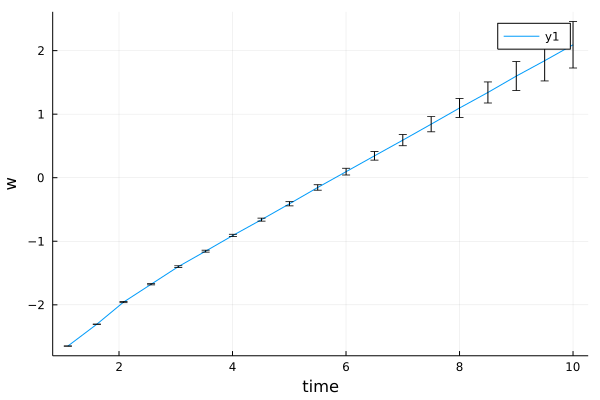
\includegraphics[width=\textwidth]{RandomBallisticDeposition3.png}
	\label{fig:mesh3}
	\caption{w over time for total particles of 1000 and a line of L=200 is shown in this plot. The initial number of particles that are going to fall in the first time-step=10.}
\end{figure}
\end{document}
